%%%%%%%%%%%%%%%%%%%%%%%%%%%%%%%%%%%%%%%%%
% Stylish Article
% LaTeX Template
% Version 2.1 (1/10/15)
%
% This template has been downloaded from:
% http://www.LaTeXTemplates.com
%
% Original author:
% Mathias Legrand (legrand.mathias@gmail.com) 
% With extensive modifications by:
% Vel (vel@latextemplates.com)
%
% License:
% CC BY-NC-SA 3.0 (http://creativecommons.org/licenses/by-nc-sa/3.0/)
%
%%%%%%%%%%%%%%%%%%%%%%%%%%%%%%%%%%%%%%%%%

%----------------------------------------------------------------------------------------
%	PACKAGES AND OTHER DOCUMENT CONFIGURATIONS
%----------------------------------------------------------------------------------------

\documentclass[fleqn,10pt]{SelfArx} % Document font size and equations flushed left

\usepackage[english]{babel} % Specify a different language here - english by default

\usepackage{lipsum} % Required to insert dummy text. To be removed otherwise
\usepackage{graphicx}
\usepackage{biblatex}
%----------------------------------------------------------------------------------------
%	COLUMNS
%----------------------------------------------------------------------------------------

\setlength{\columnsep}{0.55cm} % Distance between the two columns of text
\setlength{\fboxrule}{0.75pt} % Width of the border around the abstract

%----------------------------------------------------------------------------------------
%	COLORS
%----------------------------------------------------------------------------------------

\definecolor{color1}{RGB}{0,0,90} % Color of the article title and sections
\definecolor{color2}{RGB}{0,20,20} % Color of the boxes behind the abstract and headings

%----------------------------------------------------------------------------------------
%	HYPERLINKS
%----------------------------------------------------------------------------------------

\usepackage{hyperref} % Required for hyperlinks
\hypersetup{hidelinks,colorlinks,breaklinks=true,urlcolor=color2,citecolor=color1,linkcolor=color1,bookmarksopen=false,pdftitle={Title},pdfauthor={Author}}

%----------------------------------------------------------------------------------------
%	ARTICLE INFORMATION
%----------------------------------------------------------------------------------------

\JournalInfo{Applied Machine Learning Fall 2017} % Journal information
\Archive{} % Additional notes (e.g. copyright, DOI, review/research article)

\PaperTitle{Semester Project} % Article title

\Authors{Soutri Mukherjee\textsuperscript{1}, Ashay Sawant\textsuperscript{2}} % Authors
\affiliation{\textsuperscript{1}\textit{Computer Science, School of Informatics and Computing, Indiana University, Bloomington, IN, USA}} % Author affiliation
\affiliation{\textsuperscript{2}\textit{Data Science, School of Informatics and Computing, Indiana University, Bloomington, IN, USA}} % Author affiliation
\affiliation{*\textbf{Corresponding author}: soumukh@iu.edu, ahsawant@umail.iu.edu} % Corresponding author

\Keywords{Regression --- XGBoost --- Random Forest} % Keywords - if you don't want any simply remove all the text between the curly brackets
\newcommand{\keywordname}{Keywords} % Defines the keywords heading name

%----------------------------------------------------------------------------------------
%	ABSTRACT
%----------------------------------------------------------------------------------------

\Abstract{
 Most of the insurance providers calculate the rate based on the demographics and accident history. Failure in accurately predicting insurance claims, results in extravagant insurance cost. Porto Seguro, one of the largest auto insurance companies in Brazil, has collaborated with Kaggle's Machine Learning Community to build a model that predicts the probability that a driver will initiate an auto insurance claim in the next year.
}

%----------------------------------------------------------------------------------------

\begin{document}

\flushbottom % Makes all text pages the same height

\maketitle % Print the title and abstract box

\tableofcontents % Print the contents section

\thispagestyle{empty} % Removes page numbering from the first page

%----------------------------------------------------------------------------------------
%	ARTICLE CONTENTS
%----------------------------------------------------------------------------------------

\section*{Introduction} % The \section*{} command stops section numbering

\addcontentsline{toc}{section}{Introduction} % Adds this section to the table of contents
The major drawbacks of most insurance companies is that they  unfairely charge every client, the same amount of insurance bill, even though some of them are cautious enough to not face a single accident for years. Thus, inaccuracies in such insurance company’s claim predictions raise the cost of insurance for good drivers and reduce the price of the bad ones.  Porto Seguro , a property and personnel insurance company of Brazil , has decided to address this issue. They have approached Kaggle , one of the world’s most elite Machine Learning company  , in search of more powerful machine learning techniques than the ones they have already implemented.\\

Kaggle has turned this problem into a challenge for the fellow Kagglers. The key to winning this challenge is to build a model that predicts the probability that a driver will initiate an auto insurance claim in the next year. The most accurate prediction will allow the company to customize the prices and make the auto insurance company more accessible to more drivers.\\

This challenge can be found on the official Kaggle page. The link to the same is \href{https://www.kaggle.com/c/porto-seguro-safe-driver-prediction}{here.}\\Kaggle has provided us with training dataset, testing dataset, sample submission file.These datasets consist of binary features as well as categorical features. Feature names  that have bin as postfix indicate the binary features while those with cat as postfix indicate the categorical features. The features that belong to one similar groups have feature names with tags. These tags represent the group that they belong to. Ind,reg,car,calc are some group names to watch out for. Features that do no belong to any of the above designations are either continuous or categorical. The training dataset has 59 features which includes columns like id -an identifier of every row, target -prediction variable for training dataset and 57 other binary, categorical and continuous features. Training dataset contains 58 features, everything except the target feature(prediction).The target columns tells us whether a claim was filed for that policy holder or not.\\   
   

%------------------------------------------------
\section{Data Pre-Processing}
\addcontentsline{toc}{section}{Introduction} % Adds this section to the table of contents

\paragraph{} 
Data Pre-Processing is a procedure to convert raw data into an understandable format , before it can be used to perform any kind of analysis. Data preprocessing is very important due to the following reasons. Firstly,it removes all the errors or outliers from the dataset. Secondly, it handles all the missing values for each feature in our dataset.Thirdly,it performs several operations such as data extraction, cleaning and transformation to provide us with quality data.The processed data that we get as an output will have maximum accuracy,interpretability,timeliness,credibility and completeness which in turn will provide us with quality analysis. 

\subsection{Data Cleaning}

As we know, Real World Data can be pretty inconsistent and noisy\cite{2}. Presence of missing values in the features of such datasets leads to such kind of inconsistency. Having missing values in our dataset while we are using the same to analyze our model, can lead to invalid conclusions and may even challenge the credibility of our trails.Hence, it is very important to remove these missing values from our tuples. In the given dataset , the missing values are denoted by -1. Since, our dataset consist of continuous as well as discrete features, the missing values will be handled individually for each type.

Data-cleaning operation is divided in following two steps:
\begin{itemize}
	\item We have calculated the Number of NA's per feature of Training and Testing Dataset.The following plots show the percentage of NA values in all the features of testing ad training dataset.\\
	\begin{figure}[h]
	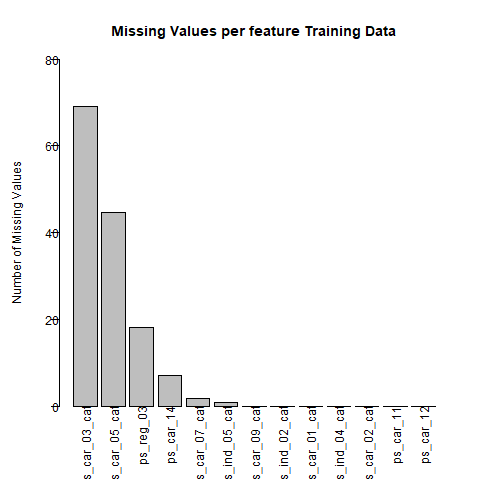
\includegraphics[width=1\columnwidth]{plots/train_missing.png}\centering
	\caption{Missing values in Training Dataset}
	\end{figure}\\
	
	\begin{figure}[h]
	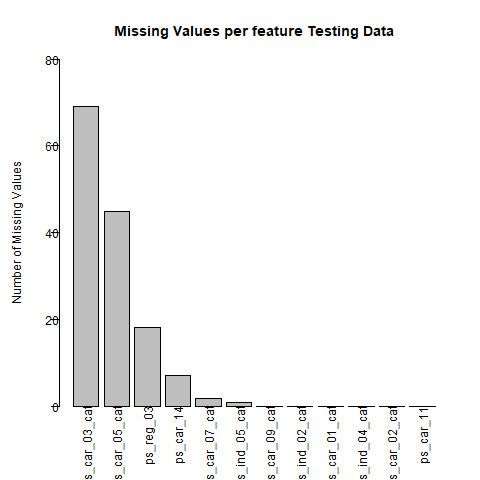
\includegraphics[width=1\columnwidth]{plots/test_missing.png}\centering
	\caption{Missing values in Testing Dataset}
	\end{figure}
	
	From the above plots, we see that pscar03cat, pscar05cat, psreg03 are top three features with most number of NA's. We have considered 40 percent as our threshold value and removed any feature having more than 40 percent NA values. Hence,we remove these columns from our training data as well as our testing data.\\

	\item At the second stage, we are handling the missing values from the remaining features in the dataset. We are using Mode and Mean values as a replacement of NA because, we were looking for some central value that might represent our column without majorly impacting the overall behavior of our dataset.\\
	For the continuous features in our dataset, we replace the NA values with the mean. The NA value of each column will be the mean value of that column. This mean has to be calculated without taking the NA value into consideration. In order to do so we have converted -1 into NA and then calculated the mean for each feature.\\
	For categorical features, we replace the NA values with the mode. The Mode is the value that has the maximum frequency in that particular column.\\
	
\end{itemize}
\subsection{Handling Imbalance Classification}
Imbalance Classification problem occurs when one class outnumbers the other class by large proportion. Our training data is consist of 595212 data-points each of them belong to either of two classes (1's or 0's). Number of training examples in each class and percentage of total training example in each class is as below:\\
\begin{center}
\begin{tabular}{| c | c | c |}
 Class & 1's & 0's \\ 
 Count & 21694 & 573518 \\  
 Percentage & 3.644\% & 96.356\%    
\end{tabular}
\end{center}

As we can see in table above, only around 3\% of the total training examples belong to the class with target = 1. Large imbalance in the dataset like this can cause a problem while regression, as performance of classifiers is biased towards majority class. Additionally, Machine Learning Algorithms try to minimize overall error to which minority class will contribute very less, which will lead to local minimum solution.\\
\paragraph{}
There are many workarounds to handle class imbalance problem. We have tried three types of sampling method to deal with imbalance class issue.
\begin{itemize}
    \item Undersampling:\\
    As the name suggest, this method reduces the number of observations from majority class by randomly sampling observation to make the dataset balance. But problem with this approach is as we are removing observations from training data, we can lose important information.
    \item Oversampling:\\
    This method works with minority class, and replicates the observation randomly from it to balance the training dataset. This method is also known as Upsampling. This approach does not lead to any information loss, but as we are replicating observation from minority class, it can lead to over-fitting the model.\\ 
    \item Mixedsampling:\\
    Mixed sampling is the mixture of Over and Under sampling. In this approach, minority class is oversampled with replacement and majority class is undersampled without replacement. 
\end{itemize}


\subsection{Data Transformation}

Data transformation is a set of functions applied over the given dataset to improve it’s interpretability. Data transformation merely changes he range of data without affecting it’s distribution. \\

For our dataset we have applied Z-Score normalization for the transformation. Normalization is nothing but scaling  of data in such a way that the minimum value is 0 and the maximum value is 1. The normalized value of every data in the dataset is calculated by subtracting the mean of the column that data  belongs to from the data and dividing the output by  the standard deviation of that column.This form of normalization also handles the existing outliers.


\subsection{Data Reduction}
Data Reduction is the technique of reducing the number of attributes or tuples from the main dataset without removing too much of information. Data Reduction helps in viewing the data at a lower dimensionality. Data Reduction can be performed either by selecting subset of features for analysis or by merging old features to create a new set of features. For our datasets, we have performed Data Reduction in two stages: 
\begin{itemize}
	
	\item{\textbf{Feature Reduction using Correlation:}}\\
	In the first stage we calculate the correlation between all the feature from Dataset.
	\begin{figure}[h]
	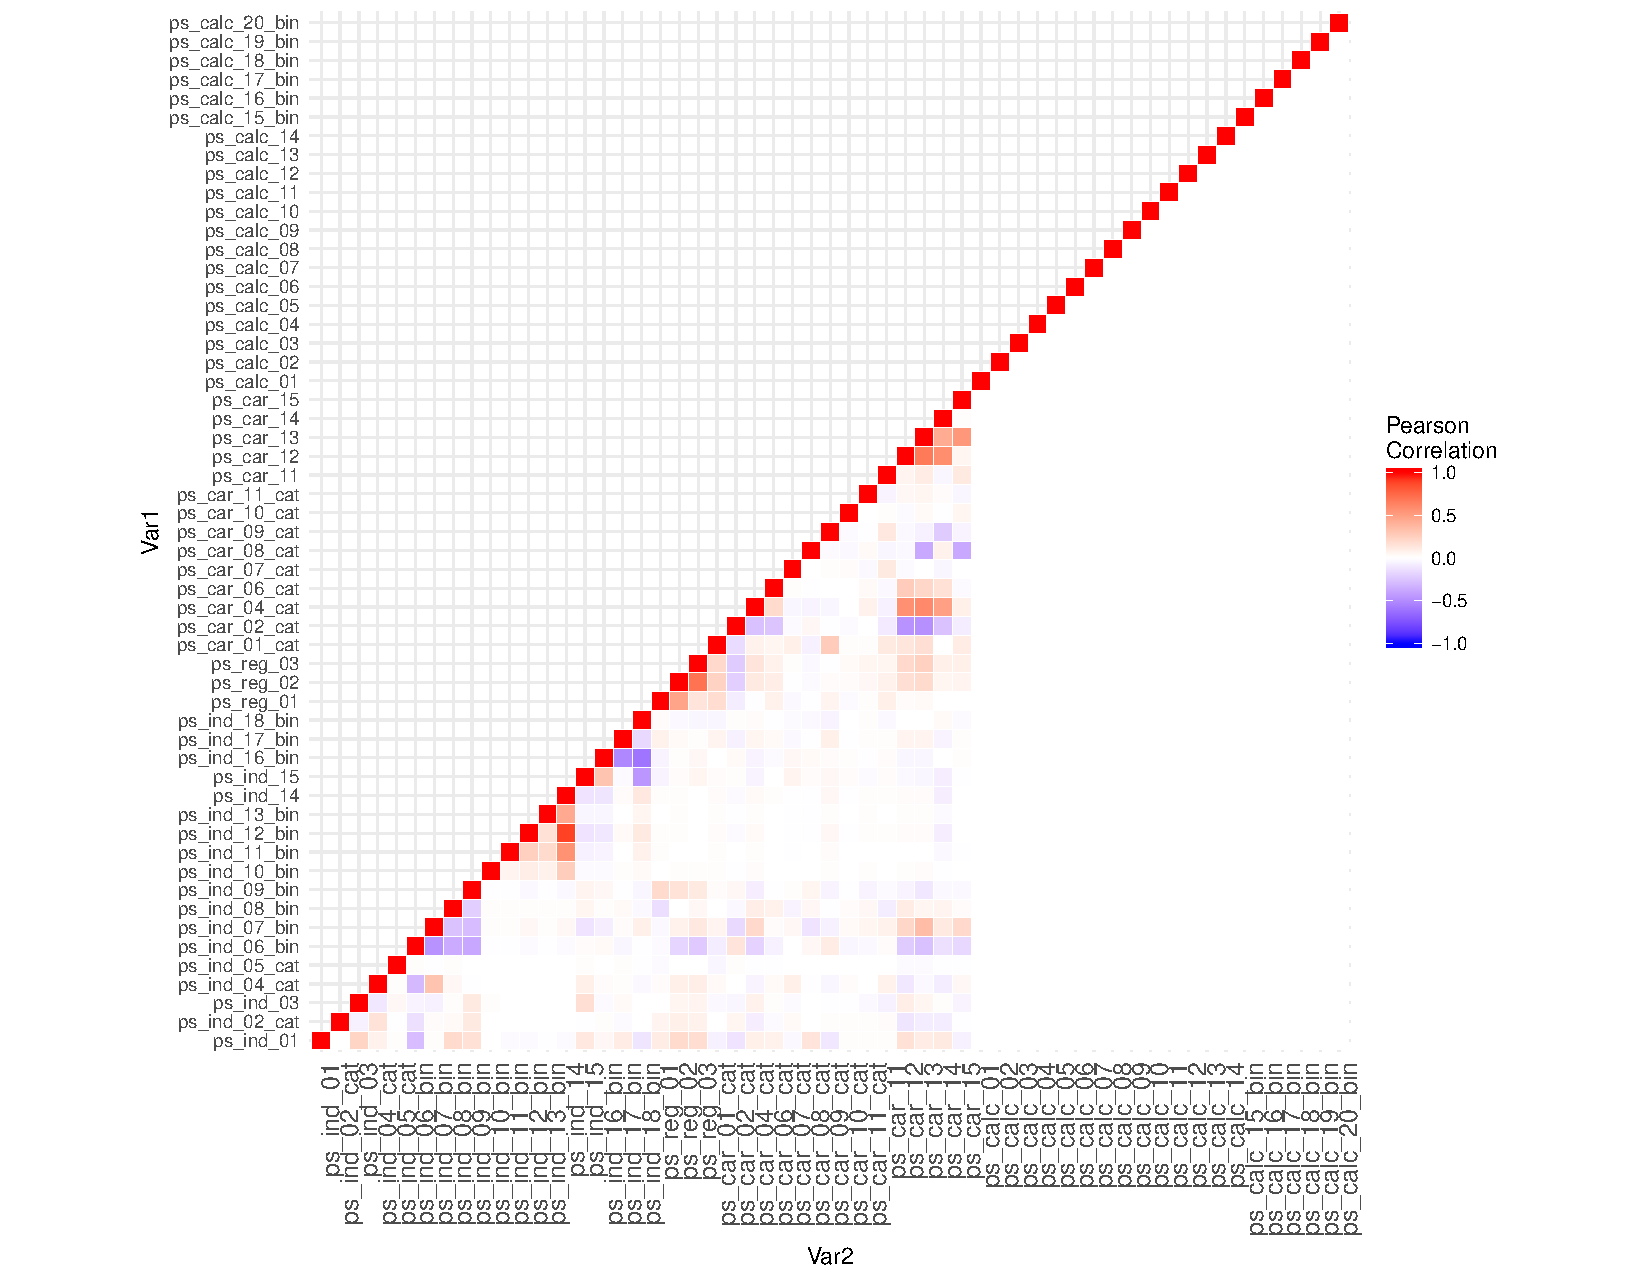
\includegraphics[width=1.1\columnwidth]{plots/corr_heat_map.pdf}\centering
	\caption{Correlation Plot of all Features}
	\end{figure}
	\\
	The Heatmap from fig.3 shows the correlation of each feature with every other feature. Hence,we can deduce that features having postfix as car or ind are highly correlated  whereas the ones with postfix as calc has negligible correlation\cite{1}. So, in order to convert the existing dataset to a lower dimensions, we drop the features with low correlation. In this case, features with calc as the postfix are the ones that need to be removed.

	\item{\textbf{Data Reduction by Feature Selection:}}\\ 
	Feature selection is the process of selecting a set of features that has maximum relevance to the predictive model. In Feature selection, we apply methods to add or drop attributes from the dataset without actually changing them. The attributes that are dropped from the dataset are either redundant, irrelevant or do not contribute to the accuracy of the predictive model. There are three classes of feature selection algorithm namely Filter Method, Wrapper Method and Embedded Methods\cite{5}.\\
	We have used filter method for feature selection in our implementation. Filter method applies statistical measures for scoring each feature. The features are then ranked according to their score and are selected or ignored based on these ranks. Gradient Boosting and Random Forest are two algorithms under filter method that we have implemented for feature selection.


\end{itemize}

\newpage
\section{Algorithm and Methodology}
\subsection{XGBoost}\\
XGBoost(eXtreme Gradient Boosting) is an advanced implementation of gradient boosting algorithm. Boosting is sequential processing technique which works on the principle of ensemble. It gives improved prediction by combining multiple weak learners. At $n^{th}$ instant, the model outcomes are weighed based on previous instant $n-1^{th}$. The outcomes which are predicted correctly gets a lower weight whereas miss-classified predictions get higher weights.\\
Highlights of XGBoost:
\begin{itemize}
    \item[1] We have used \textbf{xgboost} package of R. Computational part of xgboost method is implementated in C++ and it can be multithreaded on single machine.
    \item[2] Customized Objective: XGBoost can be used to train model with custom objective function. Hence, user can define custom objective to improve the model.
    \item[3] Early Stopping: While building the decision trees, if the number of trees to be build is large then waiting time increases. Early stopping parameter when set, XGBoost will terminate the training process if performance is getting worst.  
    \item[4] Handle Missing Values: XGBoost uses soft-coding method to handle missing values. When it encounters a missing value while splitting, it assigns direction instead of numerical value to the missing value.
    \item[5] Feature Importance: XGBoost tries to find best feature and splitting point to optemize the objective function. It calculates the information gain over the feature to decide feature importance.
\end{itemize}
    \begin{figure}[h]
	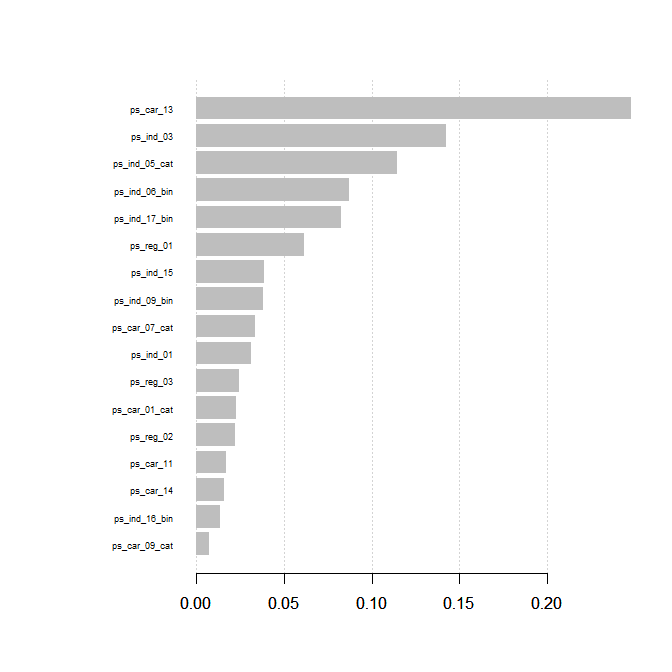
\includegraphics[width=1\columnwidth]{plots/xgboost_feature_importance.png}\centering
	\caption{Feature Importance using XGBoost}
	\end{figure}

As mentioned earlier, we have used XGBoost Algorithm to calculate the feature importance and then select only those important feature for regression. As we can see in figure 4, we have selected these 17 important features to train regression model over training data.\\  

\subsection{Logistic Regression}
Logistic Regression is used when target variable is dichotomous variable, that means when training data is consist of only two classes. We have primarily used Logistic Regression to find the target variable for test dataset.\\
\paragraph{}
Right after cleaning data by removing null values, we have used Logistic Regression to access the performance of the algorithm on data with any feature engineering. We have plot ROC plot to find the area under curve and \% Error in validation dataset.\\
    \begin{figure}[h]
	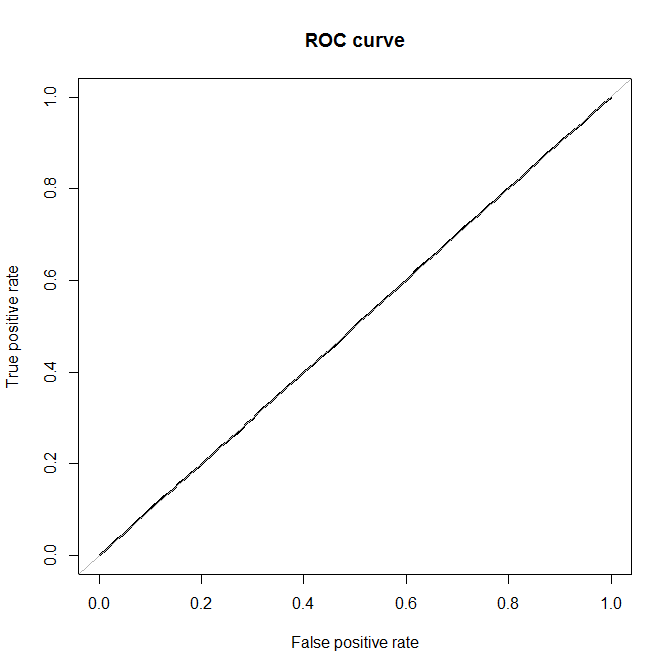
\includegraphics[width=0.8\columnwidth]{plots/ROC_logistic.png}\centering
	\caption{ROC Logistic Regression}
	\end{figure}\\
	
	We are getting 96.33\% success rate over validation dataset, which is above expectations. But, as we can see in figure 5, the Area under curve for fitted model is 0.5 which is too small. Hence, we can conclude that, due to imbalance class problem, model is over-fitted.\\
	\paragraph{}
	Further, we processed the dataset to handle imbalance class problem using the three sampling methods.
	
	\begin{figure}[h]
	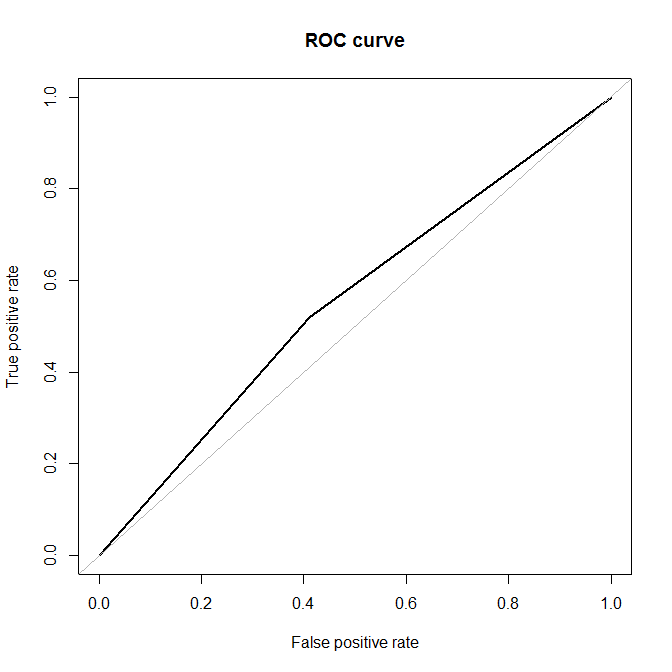
\includegraphics[width=0.8\columnwidth]{plots/ROC_under.png}\centering
	\caption{ROC of Logistic Regression on Undersampled Dataset}
	\end{figure}
	
	\begin{figure}[h]
	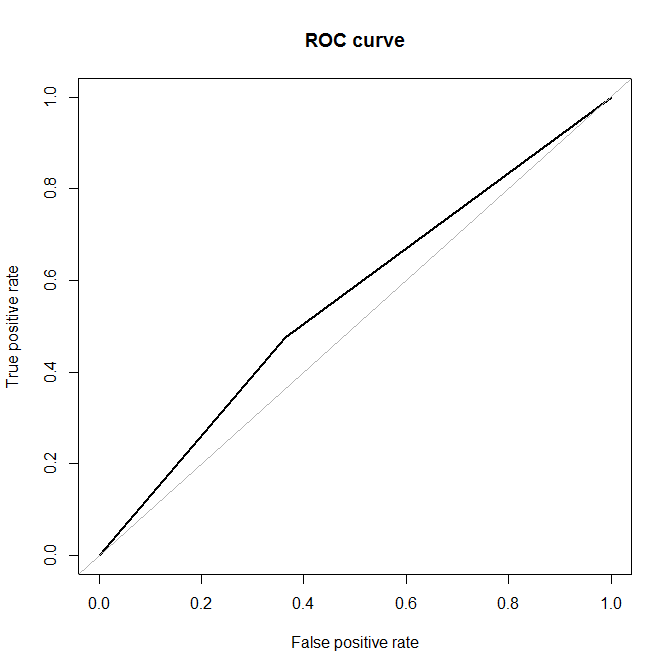
\includegraphics[width=0.8\columnwidth]{plots/ROC_over.png}\centering
	\caption{ROC of Logistic Regression on Oversampled Dataset}
	\end{figure}
	
	\begin{figure}[h]
	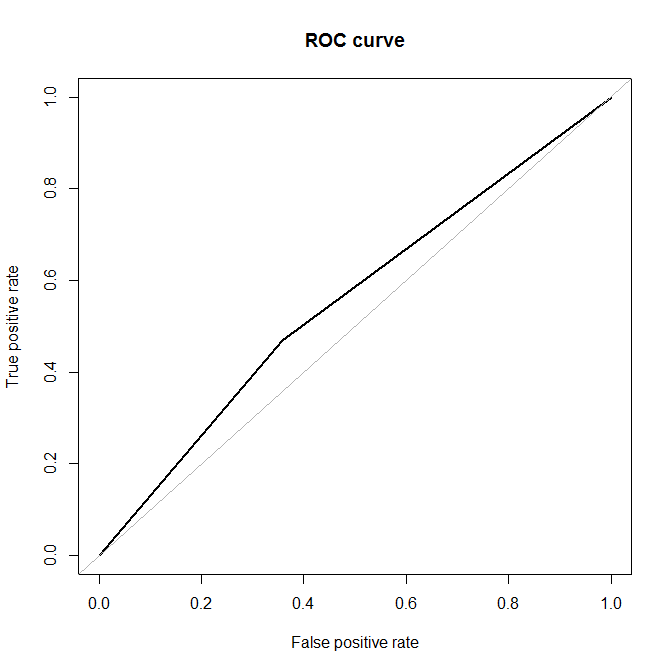
\includegraphics[width=0.8\columnwidth]{plots/ROC_both.png}\centering
	\caption{ROC of Logistic Regression on Mix-sampled Dataset}
	\end{figure}
	
	Figure 6 shows the ROC curve with Logistic Regression performed on Dataset processed with Undersampling technique. Figure 7 shows the ROC curve with Logistic Regression performed on Dataset processed with Oversampling technique. Figure 8 shows the ROC curve with Logistic Regression performed on Dataset processed with Mixsampling technique.\\
	
	After submitting the prediction on Kaggle, we have received 0.250 public score and ranked in top 3000 submissions.\\   

\newpage
\subsection{Random Forest Algorithm}
Random forests algorithm, creates multiple random decision trees using only important set of the features. It take samples from the training dataset with replacement, and trees are constructed by reducing the correlation between individual classifiers. Instead of choosing best split to construct trees, it uses random subset of features for each split. Advantage of using Random Forest Algorithm is that we don't have to prune trees to prevent over-fitting of the model on the training dataset.\\
We have used \textbf{randomForest} package for the Random Forest Algorithm. We have tuned the various parameters of the function to get better prediction.
\begin{enumerate}
\item[\textbf{1.}] ntree = 100. Number of trees to grow. This should not be set to too small a number, to ensure that every input row gets predicted at least a few times.\\
\item[\textbf{2.}] nodesize = 5. Minimum size of terminal nodes. Setting this number larger causes smaller trees to be grown.\\ 
\item[\textbf{3.}] mtry = 10. Number of variables randomly sampled as candidates at each split.\\
\end{enumerate}
We trained Random Forest Algorithm with the above parameters, the gave the accuracy of 96.3\% on the training data.\\

\begin{figure}[h]
	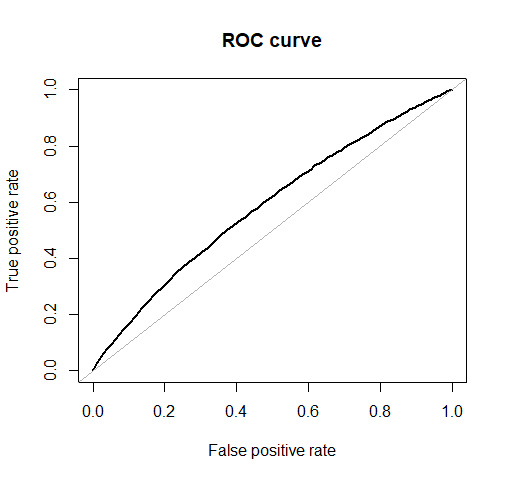
\includegraphics[width=0.8\columnwidth]{plots/ROC_random_forest.png}\centering
	\caption{ROC of Random Forest Algorithm}
	\end{figure}
	
We plot the ROC curve for Random Forest Algorithm. As we can see in figure 9, it gave Area Under Curve (AUC) = 0.588\\


Random Forest algorithm can also be used to calculate feature importance. We have selected following 20 features based on feature importance.\\
\begin{figure}[h]
	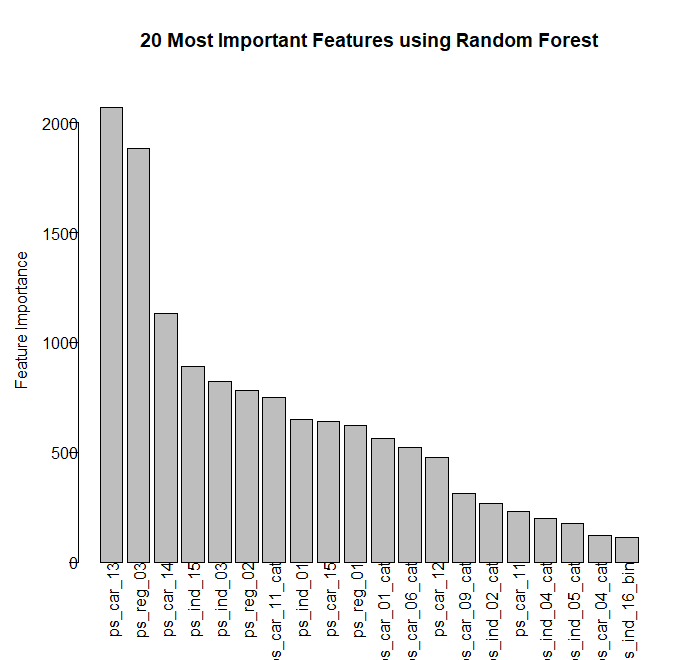
\includegraphics[width=0.8\columnwidth]{plots/rf_feature_importance.png}\centering
	\caption{Feature Importance using Random Forest Algorithm}
	\end{figure}

We again tried to train model using Logistic Regression on the above 20 features. It gave 90\% accuracy on validation dataset. Further we plot ROC curve to find Area Under Curve(AUC).\\
\begin{figure}[h]
	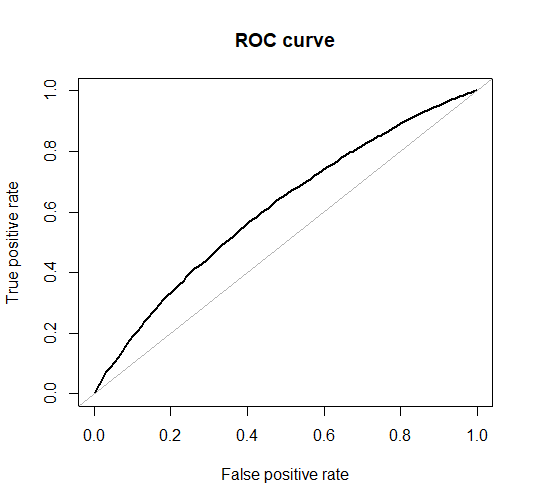
\includegraphics[width=0.8\columnwidth]{plots/ROC_RF_LOG.png}\centering
	\caption{ROC curve using Logistic Regression with Random Forest for Feature Importance}
	\end{figure}
	
With the AUC = 0.611, we predicted the target variable for test dataset. Upon submission, we got a score of 0.26717.\\


\section{Summary and Conclusions}
Thus, we have solved the Porto Seguero's challenge. We summarize our work as follows: We have analyzed the dataset and have performed Data Cleaning and Transformation at the initial stage. Then we have applied XGBoost and Random Forest Algorithm to find the feature importance and hence reduce the dimensionality of dataset. This reduced dataset is then used to train the model using logistic regression and random forest algorithm. We also compared the above mentioned algorithm by plotting ROC graphs. From the plots, we found that area under the curve for Random Forest algorithm with logistic regression is maximum. Hence, we conclude that Random Forest Algorithm for feature importance and Random Forest Algorithm for regression   performed better than other approaches we have tried.\\ 


\begin{thebibliography}{9}
\bibitem{Correlation} 
Steering Wheel of Fortune
\\https://www.kaggle.com/headsortails/steering-wheel-of-fortune-porto-seguro-eda
\bibitem{DataPreprocessing} 
Markov
\\$http://www.cs.ccsu.edu/~markov/ccsu_courses/datamining-3.html$

\bibitem{XGBoost} 
XGBoost
\\https://www.r-bloggers.com/an-introduction-to-xgboost-r-package/

\bibitem{Featimp} 
Feature Importance
\\https://machinelearningmastery.com/feature-importance-and-feature-selection-with-xgboost-in-python/
 
\bibitem{featselection} 
Feature Selction
\\https://machinelearningmastery.com/an-introduction-to-feature-selection/
\end{thebibliography}

\end{document}



